\chapter{Resultados do questionário}
\label{apendice:a}

\begin{figure}[!ht]
    \centering
    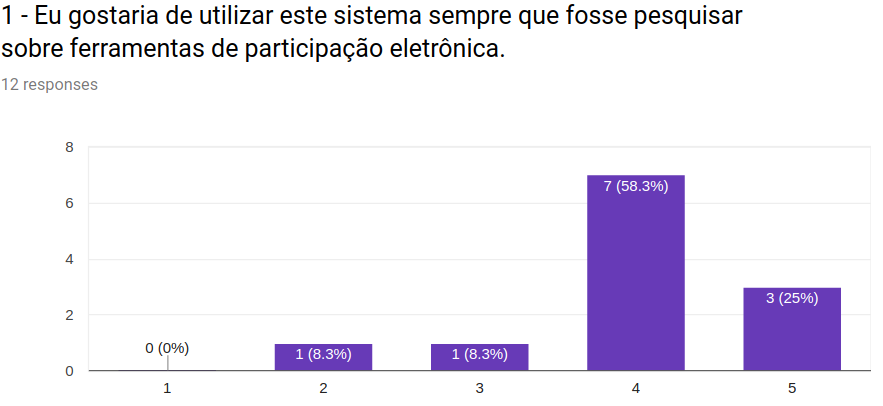
\includegraphics[scale=0.5]{./figuras/q1.png}
    \caption{Resultado do item 1.}
    \label{fig:q1}
\end{figure}

\begin{figure}[!ht]
    \centering
    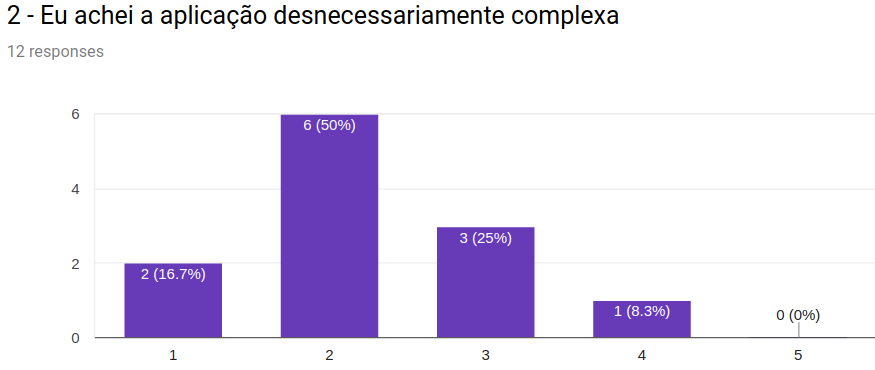
\includegraphics[scale=0.5]{./figuras/q2.png}
    \caption{Resultado do item 2.}
    \label{fig:q2}
\end{figure}

\begin{figure}[!ht]
    \centering
    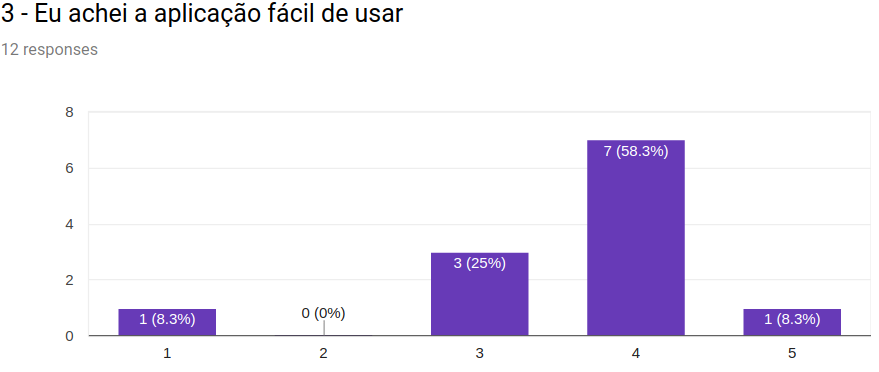
\includegraphics[scale=0.5]{./figuras/q3.png}
    \caption{Resultado do item 3.}
    \label{fig:q3}
\end{figure}

\begin{figure}[!ht]
    \centering
    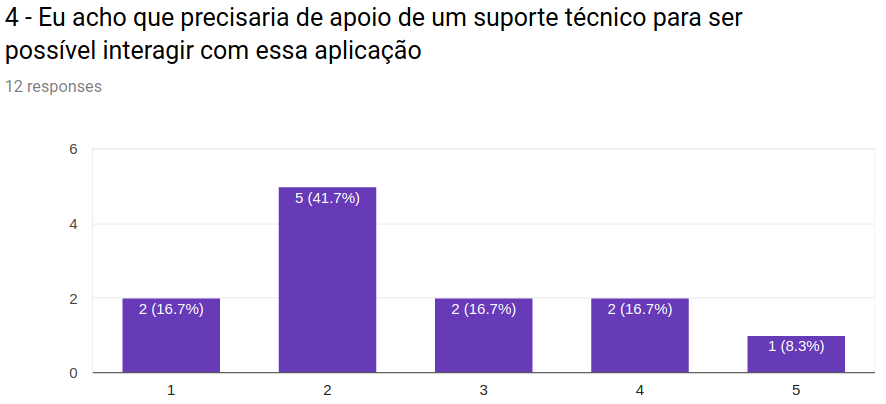
\includegraphics[scale=0.5]{./figuras/q4.png}
    \caption{Resultado do item 4.}
    \label{fig:q4}
\end{figure}

\begin{figure}[!ht]
    \centering
    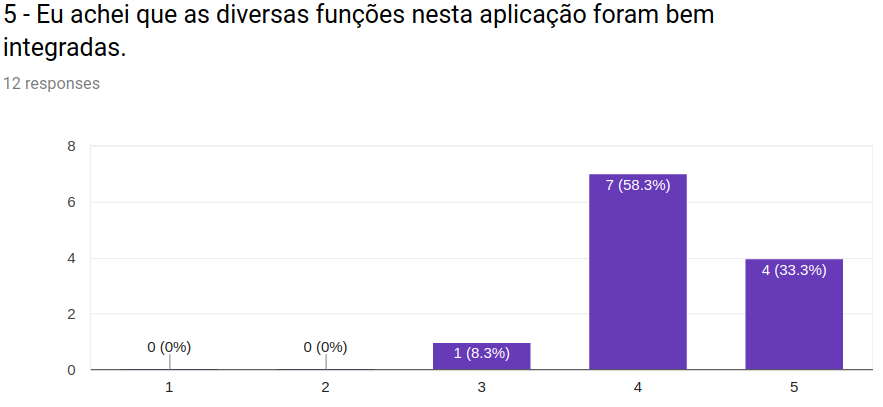
\includegraphics[scale=0.5]{./figuras/q5.png}
    \caption{Resultado do item 5.}
    \label{fig:q5}
\end{figure}

\begin{figure}[!ht]
    \centering
    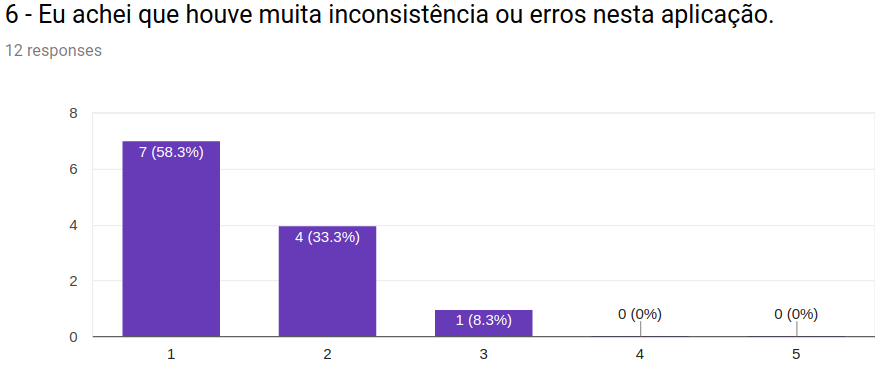
\includegraphics[scale=0.5]{./figuras/q6.png}
    \caption{Resultado do item 6.}
    \label{fig:q6}
\end{figure}

\begin{figure}[!ht]
    \centering
    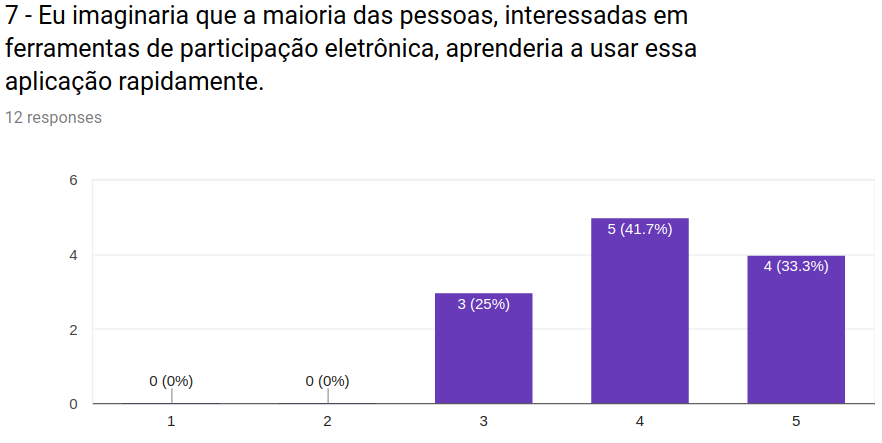
\includegraphics[scale=0.5]{./figuras/q7.png}
    \caption{Resultado do item 7.}
    \label{fig:q7}
\end{figure}

\begin{figure}[!ht]
    \centering
    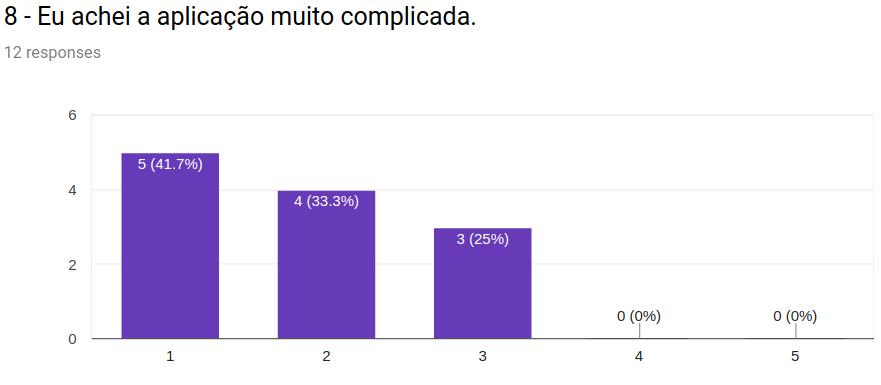
\includegraphics[scale=0.5]{./figuras/q8.png}
    \caption{Resultado do item 1.}
    \label{fig:q8}
\end{figure}

\begin{figure}[!ht]
    \centering
    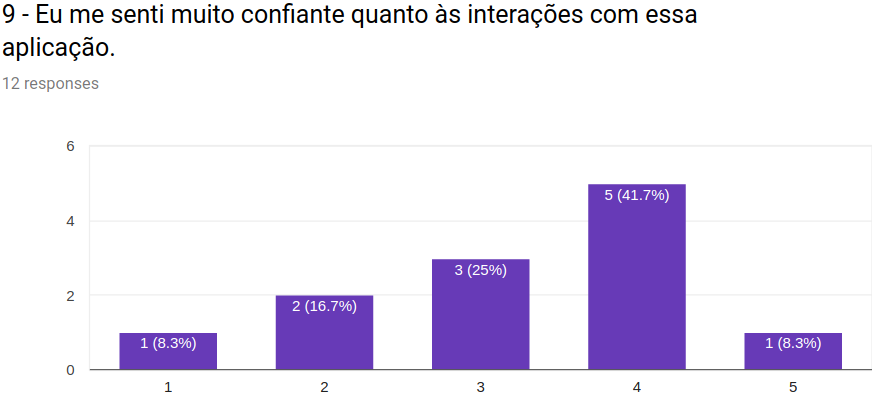
\includegraphics[scale=0.5]{./figuras/q9.png}
    \caption{Resultado do item 9.}
    \label{fig:q9}
\end{figure}

\begin{figure}[!ht]
    \centering
    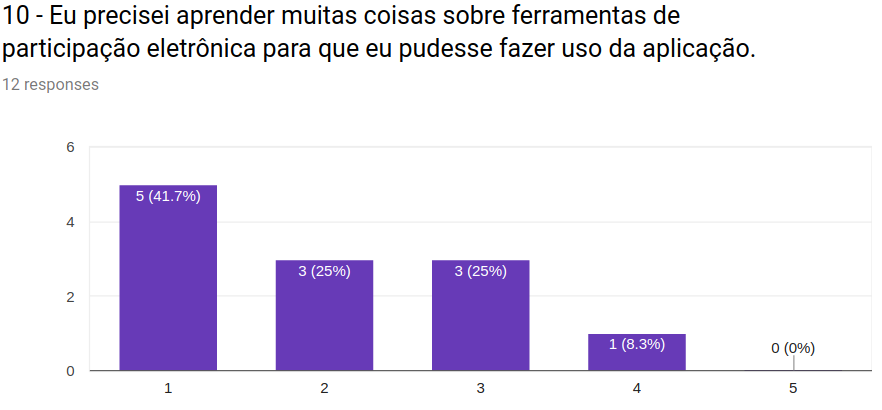
\includegraphics[scale=0.5]{./figuras/q10.png}
    \caption{Resultado do item 10.}
    \label{fig:q10}
\end{figure}